\documentclass[a4paper, 11pt]{article}
\usepackage[utf8]{inputenc}
\usepackage{graphicx} 
\usepackage{amsmath,amssymb}  
\usepackage{bm}
\usepackage{fancyhdr}
\usepackage{minted}
\usepackage[margin=3cm]{geometry} %
\usepackage[pdftex,bookmarks]{hyperref}  


\def\mytitle{Analyse d'applications réseaux}\title{\mytitle}
\def\mydate{Février 2023}\date{\mydate}
\def\myauthor{LINFO1341}\author{\myauthor}

\lfoot{} %
\cfoot{} %
\rfoot{\thepage} %
\lhead{%
	\large{Mini-Internet\space\myauthor\space-- Réseaux informatiques} \\
	\small{François Michel, Maxime Piraux, Aurélien Buchet, Olivier Bonaventure}
}
\chead{} %
\rhead{%
	\large\mydate%
}

\pagestyle{fancy}

\title{Mini-Internet: Gérer le routage d'un AS de A à Z.}
\author{François Michel \and Maxime Piraux \and Aurélien Buchet \and Olivier Bonaventure}
%\date{}

\begin{document}
\maketitle
\tableofcontents

\section{Contexte}

L'organisation dans laquelle vous travaillez vous demande
de mettre en place un Autonomous System (AS) de transit.
En tant que responsable du réseau, votre rôle
de configurer entièrement le réseau de l'organisation.
Vous êtes donc aux commandes d'un AS complet
dont vous allez configurer les routeurs pour que les utilisateurs
et serveurs de votre organisation puissent communiquer entre eux
(routage intradomaine) et qu'ils aient tous accès à Internet
(routage interdomaine).

\begin{figure}
    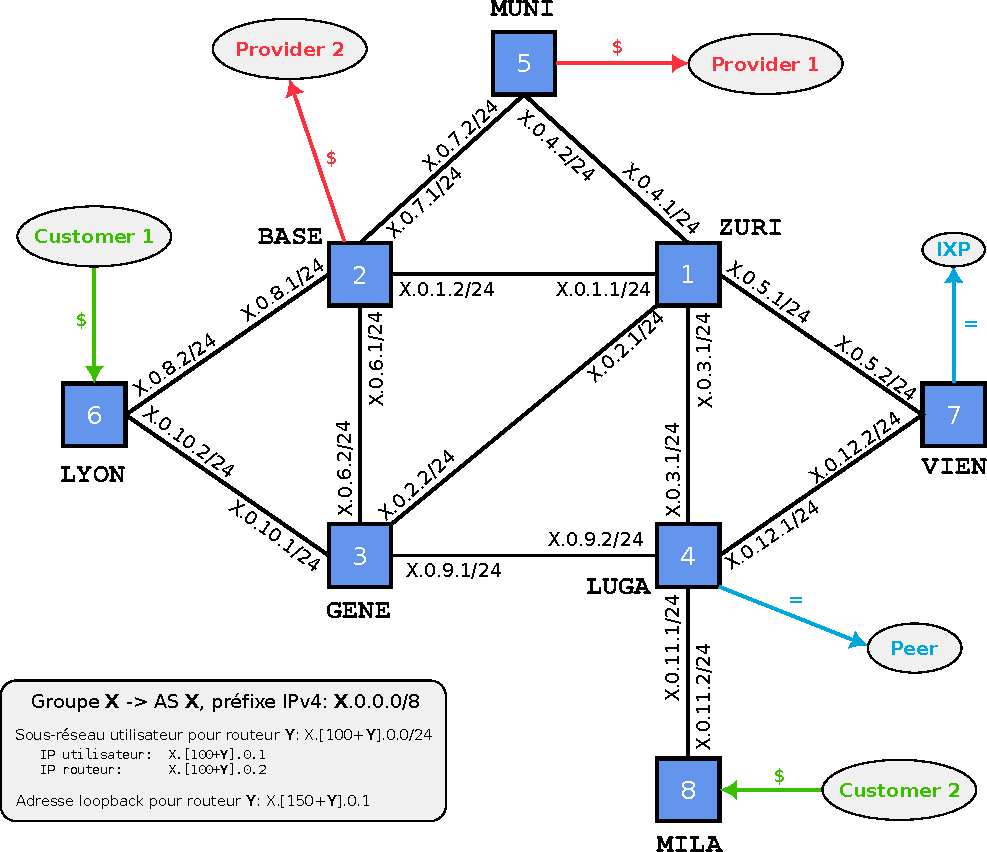
\includegraphics[width=\linewidth]{figures/topo}
    \caption{Topologie et plan d'adressage de votre AS.}
    \label{fig:topo}
\end{figure}

La Figure~\ref{fig:topo} illustre le réseau interne de votre organisation.
Il comporte 8 routeurs dont quelques uns sont connectés avec d'autres AS
appartenant à d'autres organisations. Certains d'entre eux sont
vos fournisseurs d'accès réseau (Provider): votre organisation
les paye pour qu'ils vous garantissent un accès à Internet.
D'autres sont vos clients (Customer): ils vous payent pour que
votre organisation leur garantisse un accès à Internet.   
Dans votre réseau, les routeurs \texttt{MUNI} et \texttt{BASE}
sont connectés à vos deux Providers et les routeurs \texttt{LYON}
et \texttt{MILA} sont connectés à vos deux Customers.

Certains de vos routeurs ont des liens de peering: ce sont
des liens à coûts partagés (shared-cost) établis avec d'autres AS.
Votre routeur nommé \texttt{LUGA} est connecté à un autre AS par un
lien shared-cost tandis que votre routeur nommé \texttt{VIEN} est
connecté à un Internet eXchange Point (IXP). Les IXPs sont des points
d'interconnexion entre plusieurs AS différents. Un lien avec un IXP
est à voir comme un lien shared-cost classique.

Les routeurs fournissent l'accès réseau aux divers équipements de votre
organisation (laptops, smartphones, serveurs, etc.). Pour simplifier
le projet, chacun de vos routeurs ne sera en pratique connecté qu'à un
seul appareil auquel il fournira l'accès réseau.

Vous utiliserez des outils standards pour configurer le réseau de votre
AS: OSPF (link-state routing)~\cite{rfc2328} pour le routage interne de votre AS et
BGP~\cite{rfc4271} pour le routage externe. La suite logicielle
FRRouting\footnote{\url{https://frrouting.org/}} permet de configurer
et de gérer ces deux protocoles simultanément.


\section{Se connecter à votre AS}

Votre AS tourne dans une des 4 instances de mini-Internet. Il
faut vous y connecter via \texttt{ssh} en passant par la passerelle
\texttt{studssh} en exécutant la commande suivante:
\begin{minted}{bash}
    ssh -J <user>@studssh.info.ucl.ac.be -p <port> root@<ip>
\end{minted}
où \texttt{<user>} est votre identifiant INGI, \texttt{<ip>} est
l'adresse IP de votre instance mini-Internet et \texttt{<port>}
= \texttt{2000 + <as-number>}.

Par exemple, si votre nom d'utilisateur INGI est \texttt{anna},
que votre instance mini-internet est sur l'adresse IP
\texttt{130.104.42.43} et que votre numéro d'AS est le 13,
vous pourrez vous connecter à votre AS avec la commande suivante:

\begin{minted}{bash}
    ssh -J anna@studssh.info.ucl.ac.be -p 2013 root@130.104.4.5
\end{minted}

Vous serez alors connecté à votre AS mini-Internet en utilisant
le mot de passe que vous aurez reçu en privé.

\subsection{Se connecter aux routeurs et aux appareils connectés}

Une fois dans votre AS, vous avez accès à tous les routeurs et les
appareils qui y sont connectés. Pour ce faire, vous pouvez utiliser
l'exécutable \texttt{goto.sh} disponible sur votre AS.
\texttt{./goto.sh <router-name> router} vous connectera à l'interface
du routeur, tandis que \texttt{./goto.sh <router-name> host} vous
connectera à l'interface Linux de l'appareil utilisateur directement
connecté au routeur indiqué.
Par exemple, pour vous connecter au routeur \texttt{MILA}, il suffit
de taper la commande suivante dans votre AS:

\begin{minted}{bash}
    ./goto.sh MILA router
\end{minted}


Vous arriverez alors sur l'invite de commande FRRouting qui vous
permettra de configurer le routeur MILA.
Il vous faudra alors prendre connaissance des bases de l'interface
en lignes de commandes de FRRouting. Les commandes nécessaires
à la configuration de votre routeur sont décrites sur la documentation
officielle de 
mini-Internet\footnote{\url{https://gitlab.ethz.ch/nsg/public/comm-net-2022-routing-project/-/wikis/2.-Tutorial/2.5-Configuring-IP-routers/2.5.1-The-FRRouting-CLI}}.
Pour se déconnecter du
routeur, il suffit de taper la commande \texttt{exit}, ce qui vous
ramènera dans l'interface principale de votre AS.
Pour accéder à l'appareil utilisateur connecté au routeur MILA, il vous
suffira de taper la commande suivante dans votre AS:

\begin{minted}{bash}
    ./goto.sh MILA host
\end{minted}

Vous arriverez alors sur l'invite de commande \texttt{bash} de l'appareil
connecté, ce qui vous permettra de configurer les adresses et routes
statiques de l'appareil pour qu'il utilise son routeur comme
passerelle par défaut. A nouveau, pour se déconnecter de l'appareil,
il suffit de taper la commande \texttt{exit} pour retourner sur
l'interface principale de votre AS.

\section{Accéder au site web de votre instance mini-Internet}

L'instance mini-Internet sur laquelle se trouve votre AS fournit un site
web qui vous donne un feedback en temps réel de l'interconnectivité
entre tous les AS tournant sur cette instance. Ce site web vous est aussi
nécessaire pour déterminer les AS auxquels vous devez vous connecter
en tant que Customer, Provider ou shared-cost. Le site web est fermé
à l'extérieur de l'UCLouvain, il vous faudra donc démarrer une passerelle
SSH pour le consulter. Cela peut se faire facilement via la commande
ci-dessous:

\begin{minted}{bash}
    ssh -L 127.0.0.1:8080:<ip>:80 <user>@studssh.info.ucl.ac.be
\end{minted}
Avec \texttt{<user>} votre nom d'utilisateur INGI, \texttt{<ip>} l'adresse IP
de votre instance mini-Internet, et \texttt{<port>} = \texttt{2000 + <as-number>}.
Après avoir exécuté cette commande, vous aurez directement accès au site web
de votre instance mini-Internet depuis votre navigateur en vous connectant
à \url{http://127.0.0.1:8080}, comme illustré par la
Figure~\ref{fig:website-screenshot}.

\subsection{Matrice de connectivité}

\begin{figure}
    \centering
    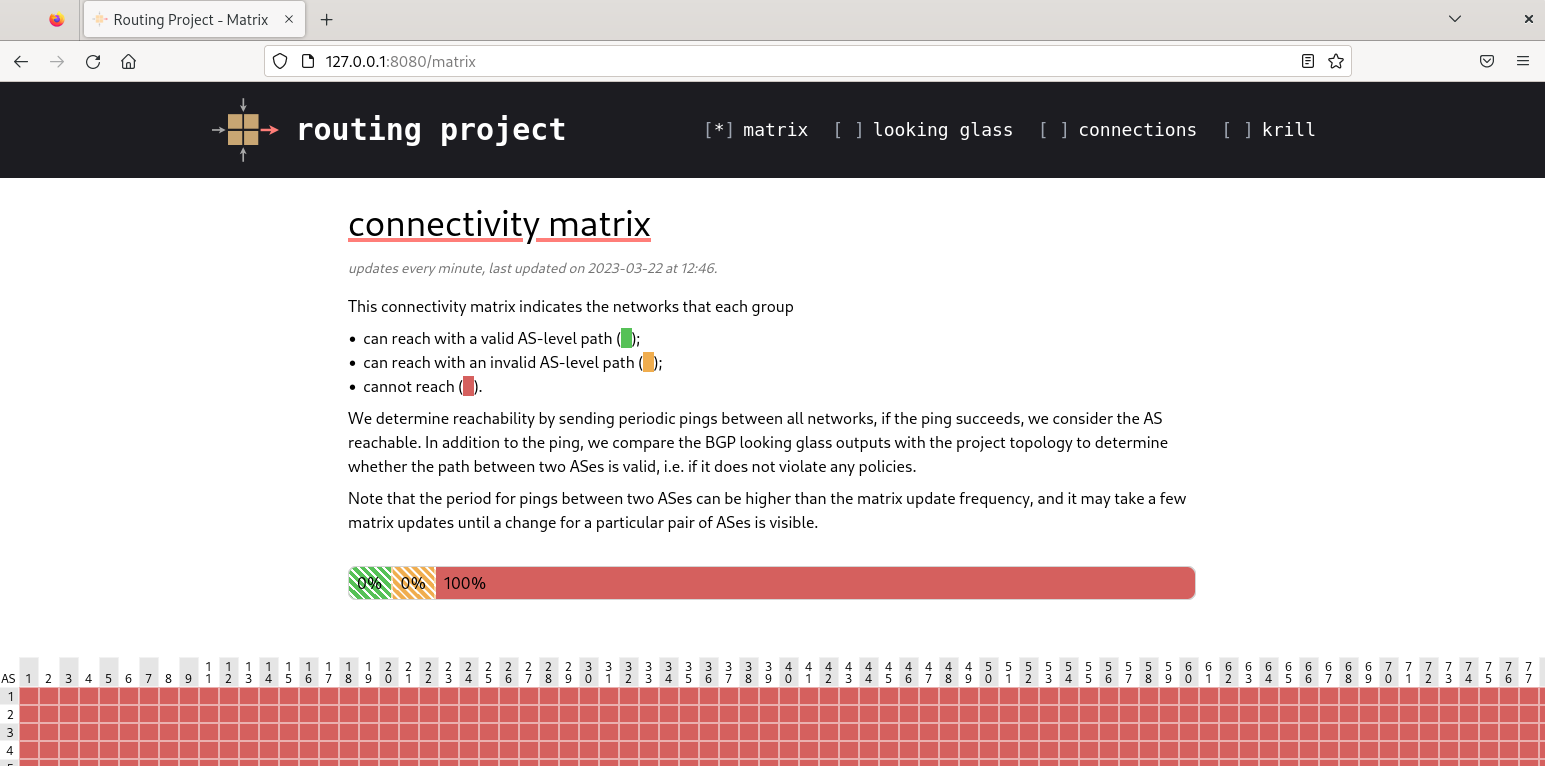
\includegraphics[width=0.8\linewidth]{figures/website-screenshot.png}
    \caption{On peut accéder au site web de l'instance mini-Internet
            en visitant la page \url{http://127.0.0.1:8080}
            une fois la passerelle démarrée.}
    \label{fig:website-screenshot}
\end{figure}

La page principale du site web de votre instance mini-Internet affiche la
matrice de connectivité de votre instance: elle indique par une couleur
l'état de la connectivité entre deux AS. L'objectif est que votre AS
obtienne une case verte pour tous les autres AS tournant sur votre instance.
Lorsque la case est rouge, cela signifie les deux AS ne peuvent pas se joindre.
Lorsque la case est orange, cela signifie que les deux AS peuvent se joindre,
mais par un mauvais chemin, ce qui signifie que les politiques de routage
interdomaine (BGP) sont mal configurées sur l'un des deux AS. Notez que la
matrice peut prendre plus de dix minutes pour se mettre à jour complètement.


\subsection{Connexions avec les autres AS}

\begin{figure}
    \centering
    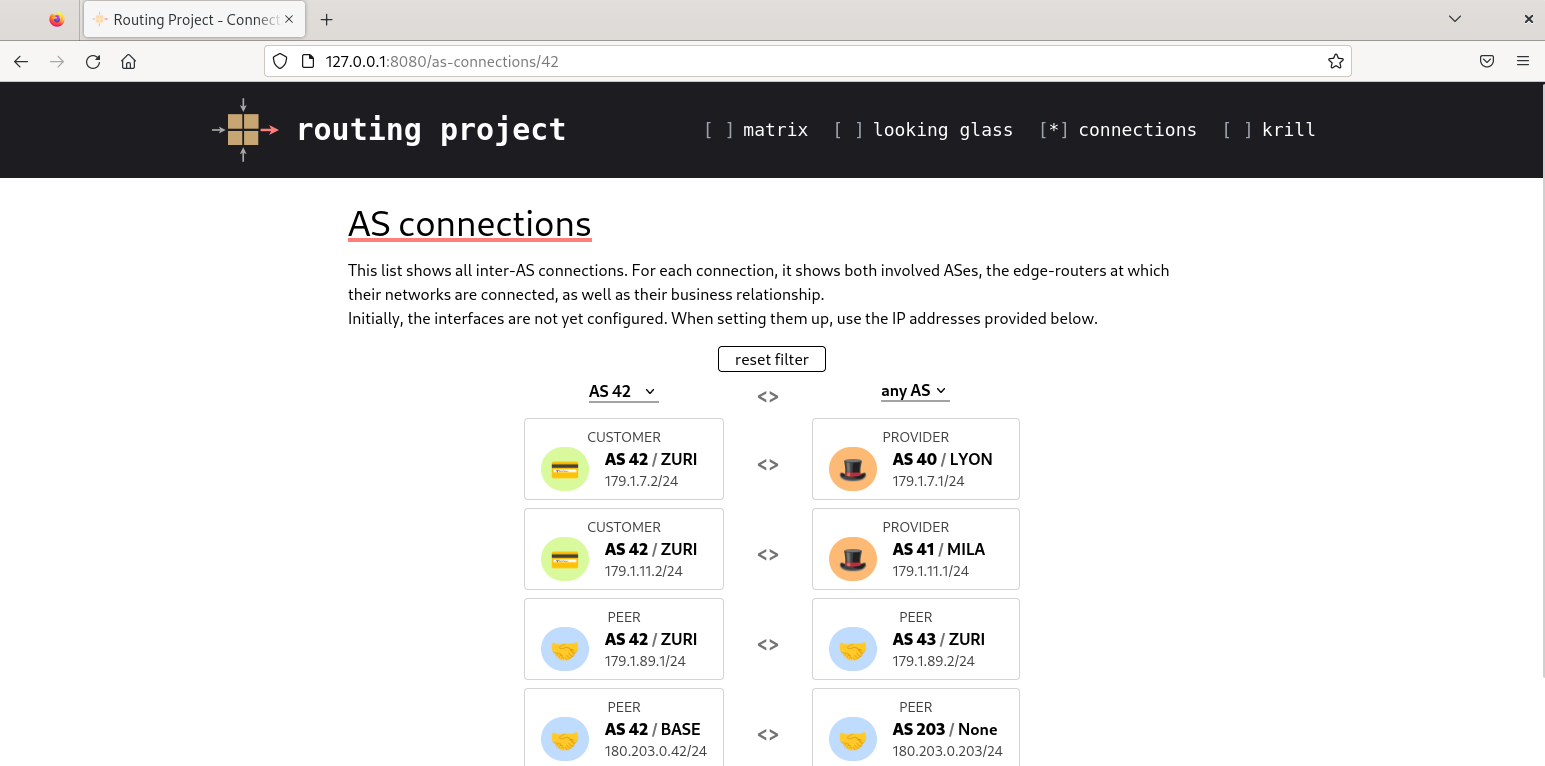
\includegraphics[width=0.8\linewidth]{figures/as-connections-screenshot.png}
    \caption{En regardant dans l'onglet \textit{connections}, l'AS 42 peut voir
    qu'il doit établir des sessions BGP avec les AS 40, 41, 43 et 203.}
    \label{fig:as-connections-screenshot}
\end{figure}

L'onglet \textit{connections} du site web vous indique avec quels AS vous
devrez établir des sessions eBGP et le type de relation que vous entretenez
avec cet AS (Provider, Customer ou Shared-Cost). La
Figure~\ref{fig:as-connections-screenshot} montre un screenshot de l'onglet
\texttt{connections} pour l'AS 42.

\subsection{Debugguer BGP avec looking glass}

\begin{figure}
    \centering
    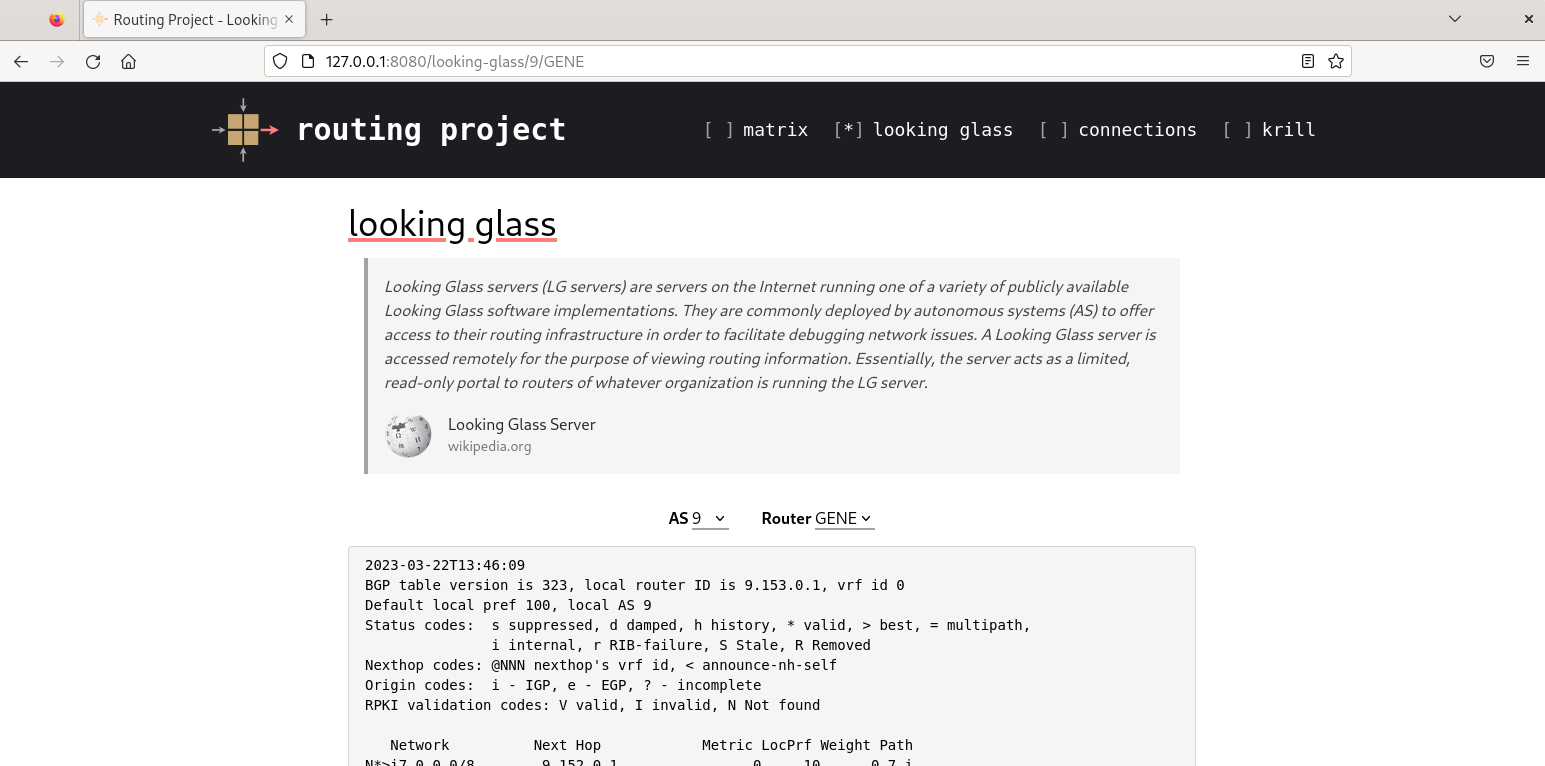
\includegraphics[width=0.8\linewidth]{figures/looking-glass-screenshot.png}
    \caption{En regardant dans l'onglet \textit{looking glass}, l'AS peut voir
    un résumé de sa configuration BGP et les possibles erreurs de configuration
    commises.}
    \label{fig:looking-glass-screenshot}
\end{figure}

L'onglet \textit{looking glass} du site web résume l'état BGP de vos routeurs,
indique leurs routes préférées et les local prefs appliquées.

De plus, en bas de page, l'onglet liste les possibles erreurs de configuration
BGP de votre AS. La Figure~\ref{fig:looking-glass-screenshot} montre un
screenshot de l'onglet \textit{looking glass}.


\section{Plan d'adressage de votre AS}\label{sec:plan-adressage}

Votre organisation dispose déjà de son plan d'adressage IPv4 qu'il
vous faudra suivre à la lettre pour configurer le réseau correctement.
Vous vous êtes fait attribuer un numéro d'AS ainsi qu'un identifiant
d'instance mini-Internet. Votre numéro d'AS est unique dans l'instance
dans laquelle vous vous trouvez. Ce numéro est utilisé pour l'adressage
IPv4 de votre réseau. Votre organisation dispose du préfixe
\texttt{X.0.0.0/8} pour ses adresses IPv4 où X est votre numéro d'AS.

La Figure~\ref{fig:topo} définit le plan d'adressage de votre organisation
dans lequel chaque routeur possède un numéro Y. Le plan d'adressage
définit un sous-réseau /24 par interface de vos routeurs.

\paragraph*{Interfaces vers un autre routeur}
Le nom des interfaces
connectées à d'autres routeurs suit le format \texttt{port\_<voisin>}
où \texttt{<voisin>} est le nom du routeur voisin auquel l'interface
est connectée. Par exemple, l'interface de \texttt{MUNI} connectée à
\texttt{BASE} porte le nom \texttt{port\_BASE}.
À chacune de ces interfaces est assigné un sous-réseau /24 qui lui permet
de communiquer avec l'autre routeur connecté à ce lien.

\paragraph*{Sous-réseau pour l'utilisateur connecté}
Chaque routeur est également doté d'une interface \texttt{host}
directement connectée
à un appareil utilisateur et fournit le sous-réseau
\texttt{X.[100+Y].0.0/24} à cet appareil utilisateur.
Dans ce sous réseau, l'adresse IP de l'hôte sera \texttt{X.[100+Y].0.1}
et le routeur possède l'adresse \texttt{X.[100+Y].0.2}. Sur le routeur
\texttt{MUNI}, l'interface \texttt{host} se verra donc affecter
le préfixe \texttt{X.105.0.0/24}. L'IP du routeur sur ce sous-réseau
sera \texttt{X.105.0.2} et l'IP de l'hôte connecté au routeur
sera \texttt{X.105.0.1}.

\paragraph*{Interface loopback}
Le routeur possède aussi
une interface \textit{loopback} nommée \texttt{lo}. Une interface loopback
est une interface virtuelle qui permet d'assigner une unique adresse
joignable via toutes les interfaces du routeur, indépendamment des
sous-réseaux assignés à ces interfaces. Cela permet à tous les autres
routeurs de le joindre en utilisant simplement l'adresse loopback.
L'adresse loopback de chaque routeur est \texttt{X.[150+Y].0.1}.
Pour le routeur \texttt{MUNI}, l'adresse assignée à l'interface
loopback sera donc \texttt{X.155.0.1}.


\section{Configuration pas-à-pas du routage de votre AS}


L'objectif du projet est de configurer entièrement le réseau de votre AS.
Cette configuration se déroule en 4 parties. Tout d'abord, l'assignation
manuelle des adresses IPs et des sous-réseaux sur les différentes interfaces
de vos routeurs. Ensuite, la configuration manuelle de l'adresse IP et de la
route par défaut sur sur les appareils connectés à vos routeurs pour qu'ils
envoient correctement leurs paquets à leur routeur.
Ensuite vient la configuration automatique du routage intradomaine
en utilisant le protocole à état de liaison OSPF, qui permettra aux routeurs
de découvrir la topologie du réseau et de construire automatiquement
les tables de routage. L'interface de FRRouting permet de configurer
facilement OSPF. Finalement, la configuration automatique du routage
interdomaine se fera avec BGP, également via l'interface FRRouting.
Cette section explique pas-à-pas les différentes étapes de configuration
du projet. Nous vous conseillons de les suivre dans l'ordre.

\subsection{Adresses IPs et sous-réseaux des routeurs}

La première partie du projet consiste à assigner correctement les
sous-réseaux sur les bonnes interfaces des routeurs en se référant au
plan d'adressage de la Figure~\ref{fig:topo} (les appareils utilisateurs
connectés à chacun des routeurs ne sont pas dessinés sur la Figure).
Par exemple, le routeur \texttt{MUNI} doit affecter le sous-réseau
\texttt{X.0.7.0/24} à son interface \texttt{port\_BASE}. Son adresse
IP sur ce sous-réseau est \texttt{X.0.7.2}. Il doit aussi affecter le
sous-réseau \texttt{X.0.4.0/24} à son interface \texttt{port\_ZURI} et
sa propre adresse IP sur ce sous-réseau sera \texttt{X.0.4.2}.

Finalement, chaque routeur doit assigner un sous-réseau spécifique sur
l'interface \texttt{host}. Par exemple,
le routeur \texttt{MUNI} devra y assigner le sous-réseau
\texttt{X.105.0.0/24}. Son adresse IP sur l'interface \texttt{host}
sera \texttt{X.105.0.2}.

Assigner les adresses IP et les sous-réseaux sur un routeur
peut être fait directement depuis l'invite de commandes
de FRRouting. Un exemple de configuration des adresses
et sous-réseaux des routeurs est disponible sur la
documentation de
mini-Internet
\footnote{\url{https://gitlab.ethz.ch/nsg/public/comm-net-2022-routing-project/-/wikis/2.-Tutorial/2.5-Configuring-IP-routers/2.5.1-The-FRRouting-CLI}}
\footnote{\url{https://gitlab.ethz.ch/nsg/public/comm-net-2022-routing-project/-/wikis/2.-Tutorial/2.5-Configuring-IP-routers/2.5.2-Configuring-router-interfaces}}
\footnote{\url{https://gitlab.ethz.ch/nsg/public/comm-net-2022-routing-project/-/wikis/2.-Tutorial/2.5-Configuring-IP-routers/2.5.3-Configure-static-routes}}
.
\subsection{Routes statiques sur les appareils connectés}

Habituellement, les appareils utilisateurs connectées à un réseau
IPv4 reçoivent une adresse et passerelle par défaut automatiquement
grâce à l'utilisation du protocole DHCP. Pour simplifier le projet,
les hôtes connectés aux routeurs seront configurés manuellement
sans DHCP. 

\paragraph*{Sous-réseau et adresse IP} 
Chaque appareil utilisateur mini-Internet devra
être configuré pour assigner son sous-réseau et son adressse IP.
Par exemple, l'appareil connecté au routeur \texttt{MUNI} se verra
assigner l'adresse IP \texttt{X.105.0.1} dans le sous réseau
\texttt{X.105.0.0/24} sur son interface \texttt{router}.
Lorsque vous accédez à un appareil utilisateur dans votre AS
(par exemple, l'hôte connecté à \texttt{MUNI} via
\texttt{./goto.sh MUNI host}), vous accédez au terminal
bash de l'appareil.
Une adresse peut être assignée à une interface réseau en utilisant
la commande \texttt{ip addr}.

\paragraph*{Route et passerelle par défaut}
Il faut maintenant indiquer à l'OS de l'appareil qu'il peut joindre
n'importe quelle autre adresse IPv4 en envoyant tous ses paquets
au routeur auquel il est connecté. Pour ce faire, il faut ajouter une
nouvelle route à la table de routage de l'appareil en utilisant
l'utilitaire \texttt{ip route}.

Un exemple de configuration d'un appareil en utilisant
\texttt{ip addr} et \texttt{ip route} peut-être trouvée dans la documentation
de mini-Internet\footnote{\url{https://gitlab.ethz.ch/nsg/public/comm-net-2022-routing-project/-/wikis/2.-Tutorial/2.2-Configuring-a-host}}.

\subsection{Routage intradomaine avec OSPF}

Vient ensuite la configuration du routage interne de votre AS.
Chaque routeur doit être configuré pour annoncer tous
les sous-réseaux de ses interfaces
via OSPF (protocole de routage à état de liaison).
Par exemple, le routeur \texttt{MUNI} devra activer
OSPF sur les interfaces \texttt{port\_BASE} et \texttt{port\_ZURI}
et devra être configuré
pour qu'il annonce les sous-réseaux \texttt{X.0.7.0/24},
\texttt{X.0.4.0/24} et X.105.0.0/24 via OSPF.
Il devra aussi annoncer son adresse loopback \texttt{X.155.0.1}
car cette dernière sera utilisée plus tard pour iBGP.
La configuration d'OSPF se fait via l'invite de commande de
FRRouting. Un exemple de configuration d'OSPF sur FRRouting
est disponible dans la documentation de
mini-Internet\footnote{\url{https://gitlab.ethz.ch/nsg/public/comm-net-2022-routing-project/-/wikis/2.-Tutorial/2.5-Configuring-IP-routers/2.5.4-Configure-OSPF}}.


\subsection{Routage interdomaine avec eBGP et iBGP}

La dernière étape consiste à établir un lien avec les autres AS
de l'Internet: il faut donc établir des sessions eBGP avec tous vos
Customers, Providers, votre Peer et l'IXP auquel vous êtes connecté.
Il faut ensuite établir des sessions iBGP en mode full-mesh avec 
tous les routeurs du réseau pour que chaque routeur prenne connaissance
des routes obtenues via eBGP. Chaque routeur maintiendra donc
7 sessions iBGP. Les sessions iBGP se font avec les adresse loopback
des routeurs, ce qui leur permet de communiquer via n'importe quelle
interface réseau.

Il faut correctement configurer vos filtres d'import en appliquant
des local-prefs correspondant à l'AS auquel le routeur est connecté.
Comme un routeur annonce l'attribut \texttt{LOCAL\_PREF} de ses routes
sur ses sessions iBGP, cet attribut \texttt{LOCAL\_PREF} peut être
facilement utilisé pour déterminer les filtres d'export également.

Prenons l'exemple du routeur \texttt{MUNI}. Ce routeur doit
établir une session eBGP avec le Provider 1 (dans cet exemple,
imaginons que Provider 1 ait l'AS numéro 42 et que le routeur eBGP
de Provider 1 s'appelle \texttt{ZURI} et ait l'IP 42.1.2.3).
\texttt{MUNI} va donc établir une session eBGP avec le routeur
à l'adresse \texttt{42.1.2.3} sur son interface nommée
\texttt{ext\_42\_ZURI}. Comme l'AS 42 est votre Provider, votre
routeur va annoncer votre préfixe (\texttt{X.0.0.0/8}) ainsi que
les préfixes apprtenant à vos clients. 
Imaginons que l'on assigne la local pref 50 aux providers, 100 aux
shared-costs et 150 aux customers. Un filtre d'export qui ne laisserait
passer que les routes des clients serait une chaîne de filtres en 3
étapes:
\begin{enumerate}
    \item Refuser les routes aux local-pref égales à 50
    \item Refuser les routes aux local-pref égales à 100
    \item Accepter toutes les routes\footnote{Il est nécessaire
    de terminer la chaine de filtres par une règle qui accepte
    toutes les routes car la politique par défaut de FRRouting est
    de refuser totues les routes qui ne sont pas explicitement
    acceptées.}
\end{enumerate}

Le routeur \texttt{MUNI} devra également établir une session iBGP
avec les 7 autres routeurs. Une session iBGP n'est pas très différente
d'une session eBGP en termes de confirugration. Voici trois points
qui distinguent une session iBGP d'une session eBGP en termes de cofiguration :

\begin{itemize}
    \item Les deux routeurs de la session possèdent le même numéro d'AS
          (votre numéro d'AS).
    \item La session s'établit entre les adresses loopback des routeurs
          (cf le paramètre \texttt{update-source} de FRRouting).
    \item Les routeurs doivent se mettre en next-hop des routes qu'ils
          annoncent (cf le paramètre \texttt{next-hop-self} de FRRouting).
\end{itemize}

Un exemple de configuration de eBGP et iBGP sur FRRouting
est disponible dans la documentation de
mini-Internet\footnote{\url{https://gitlab.ethz.ch/nsg/public/comm-net-2022-routing-project/-/wikis/2.-Tutorial/2.5-Configuring-IP-routers/2.5.5-Configure-BGP}}.


\subsubsection{Écrire les fitres d'import et d'export avec FRRouting}

\begin{figure}
    \begin{minted}[frame=single,framesep=2mm,
        baselinestretch=0.8,]{bash}
        $ # création de la route-map PROVIDER_IN (filtre d'import)
        $ # on accepte toutes les routes
        $ route-map PROVIDER_IN permit 10
        $ # on attribue la local pref d'un provider (50)
        $ set local-preference 50
        $ exit
    
        $ # création de la route-map PROVIDER_OUT
        $ # on n'exporte pas les routes des providers:
        $ route-map PROVIDER_OUT deny 10
        $ # deny si le local pref vaut 50
        $ match local-preference 50
        $ exit
        
        $ # on n'exporte pas les routes des shared-costs:
        $ # sera exécuté après le seqnum 10
        $ route-map PROVIDER_OUT deny 20
        $ # deny si le local pref vaut 100
        $ match local-preference 100
        $ exit
    
        $ # on exporte toutes les routes qui ont passé les
        $ # deux premiers filtres
        $ # sera exécuté après le seqnum 20
        $ route-map PROVIDER_OUT permit 30
        $ exit
    
        $ # on assigne la règle PROVIDER_IN en filtre d'import
        $ neighbor 42.1.2.3 route-map PROVIDER_IN in
        $ # on assigne la règle PROVIDER_OUT en filtre d'export
        $ neighbor 42.1.2.3 route-map PROVIDER_OUT out
    \end{minted}
    \caption{Configuration des filtres eBGP avec le peer \texttt{42.1.2.3}}
    \label{fig:bgp-filters}
    \end{figure}
La documentation de mini-Internet est incomplète sur la manière dont fonctionnent
les filtres d'import et d'export de BGP dans FRRouting. Cette section
explique leur fonctionnement plus en détails.

Les filtres BGP sont représentés dans FRRouting sous le terme
\textit{route-map}. Vous pouvez définir de nouvelles route-maps
et leur donner un nom avec la commande suivante dans l'invite de
configuration de BGP:


\begin{minted}{bash}
    route-map <nom> {permit|deny} <seqnum>
    <commandes-additionelles>
    exit
\end{minted}
\texttt{<name>} est le nom de votre route-map. Le mot clé \texttt{permit}
ou \texttt{deny} permet d'accepter ou de refuser la route (les
filtres d'import accepteront toujours les routes). \texttt{<seqnum>}
permet d'ajouter plusieurs règles pour une même route-map en leur attribuant un
numéro de séquence. Ces différentes
règles seront appliquées dans l'ordre de leur numéro de séquence. Seules
les routes qui rencontrent au moins un \texttt{permit} dans une route-map
seront acceptées par le filtre.
Si une route ne rencontre aucun \texttt{permit} explicite, elle ne sera
pas autorisée par le filtre. C'est pourquoi il faudra toujours au moins une
règle \texttt{permit} dans vos route-maps. Prenons l'exemple du routeur
\texttt{MUNI}. La Figure~\ref{fig:bgp-filters} illustre un exemple
de configuration des filtres d'import et d'export du routeur \texttt{MUNI}
s'il est pairé avec le routeur \texttt{42.1.2.3} de son fournisseur, l'AS 42.


\subsubsection{Sauvegarder votre configuration}

Mini-Internet étant un large système sur lequel se connectent des centaines,
d'étudiants il est primordial de sauvegarder régulièrement votre configuration
pour être résilient à de possibles pannes dues à des erreurs de configuration.

Pour ce faire, il vous suffit de vous connecter à votre instance mini-Internet
et d'exécuter la commande \texttt{./save\_configs.sh}. Ce script génèrera
automatiquement un dossier nommé \texttt{configs\_<date>\_<heure>} ainsi
qu'un fichier \texttt{zip} contenant ce même dossier.

Il vous faudra ensuite télécharger ce fichier sur votre propre ordinateur avec
la commande \texttt{scp} qui permet de faire une copie via SSH. Cela peut se faire
via la commande suivante:


\begin{minted}{bash}
    scp -P <2000+X> root@<ip>:~/configs_<date>_<heure>.zip .
\end{minted}

avec \texttt{X} votre numéro de groupe et \texttt{<ip>} l'adresse IP de votre
instance mini-Internet.

\section{Évaluation}

L'évaluation de votre projet se fera sur base de votre configuration finale.
Voici les critères qui attireront principalement notre attention:

\begin{itemize}
    \item Les hôtes attachés à chaque routeur peuvent tous se joindre,
          et ce malgré une panne d'un des liens redondants du réseau.
    \item Les hôtes possèdent la bonne adresse IP et la bonne passerelle par
          défaut (la bonne adresse IP du routeur auquel ils sont attachés).
    \item Les interfaces des routeurs sont assignées aux bons sous-réseaux.
    \item L'interface loopback du routeur est correctement configurée.
    \item Le routage intradomaine a bien été configuré sur chaque routeur
          via OSPF et est résilient aux pannes des liens redondants.
    \item Les sessions eBGP sont correctement configurées avec vos AS Customers,
          Providers et shared-costs et les politiques de routage sont 
          appliquées correctement.
    \item iBGP est correctement configuré en full-mesh de sorte que les routes
          reçues via eBGP soient bien accessible depuis n'importe quelle machine
          (hôte ou routeur) à l'intérieur de votre réseau. 
\end{itemize}

La matrice de connectivité de mini-Internet vous sera d'une très grande utilité
pour valider votre configuration eBGP et iBGP et la bonne application des
politiques de routage interdomaine.

\bibliographystyle{abbrv}
\bibliography{bibliography.bib}
\end{document}